\begin{figure}[!h]
    \centering
    \begin{subfigure}[t]{0.49\textwidth}
         \centering
         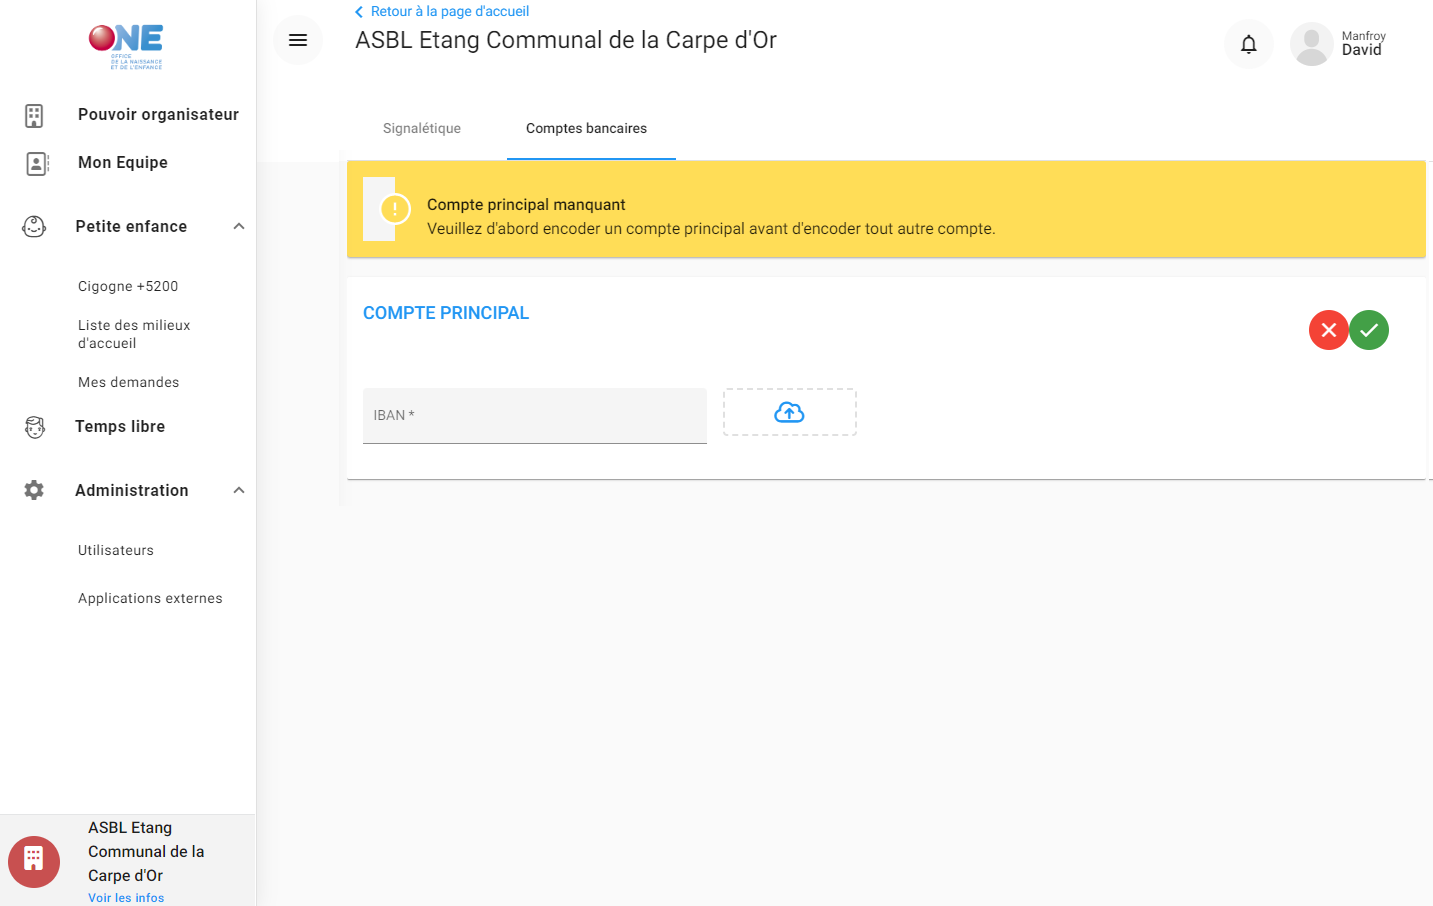
\includegraphics[width=\textwidth]{Images/gcb/gcb_compteprincipal.png}
         \caption{Aucun compte par défaut encodé}
         \label{subfig:gcb_compteprincipal}
     \end{subfigure}
     \hfill
    \begin{subfigure}[t]{0.49\textwidth}
         \centering
         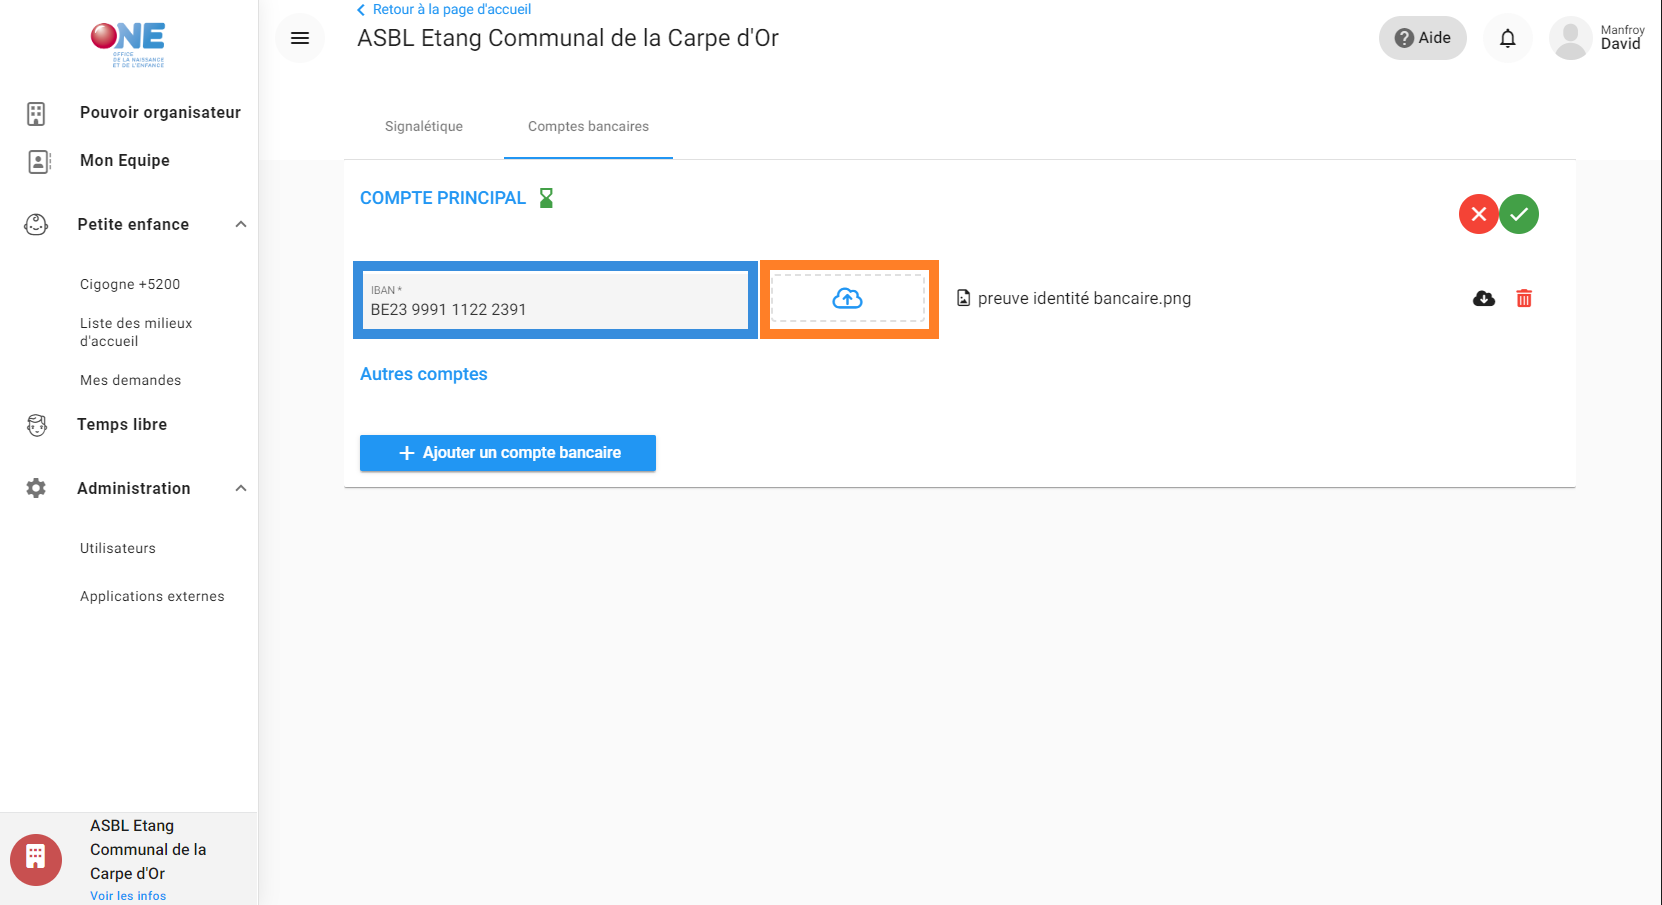
\includegraphics[width=\textwidth]{Images/gcb/gcb_compteprincipalcreate.png}
         \caption{Ajout du compte bancaire par défaut (bleu) et chargement du RIB (orange)}
         \label{subfig:gcb_compteprincipalcreate}
     \end{subfigure}
    
    \caption{Ajouter le compte par défaut}
    \label{fig:gcb_compte_par_défaut}
\end{figure}